\documentclass[11pt,oneside]{book}

% -----------------------------------------------------------------------------
% Springer Nature Textbook Architecture & Typography
% Exemplary Chapter: Mass Spectrometry Data Analysis with R
% Chapter 14: Quantitative Label-Free Proteomics: Signal Extraction,
%              Normalization, and Protein Summarization
% Author: Lucas VHH TRAN (CK-CARE Davos, Switzerland)
% -----------------------------------------------------------------------------

\usepackage{springer_monograph}

\hypersetup{
    pdftitle={Chapter 14: Quantitative Label-Free Proteomics in Mass Spectrometry},
    pdfauthor={Lucas VHH TRAN}
}

\begin{document}

% --- Chapter Title Block ---
\setcounter{chapter}{13}
\chapter{Quantitative Label-Free Proteomics: Signal Extraction, Normalization, and Protein Summarization}

\noindent
\textbf{Lucas VHH TRAN}\footnote{CK-CARE Davos, Christine K\"uhne -- Center for Allergy Research and Education, Davos, Switzerland. Email: \texttt{lucas.tran@ck-care.ch}}\\
\rule{\textwidth}{0.8pt}

\begin{abstract}
\noindent
Label-free quantification (LFQ) represents the dominant and most versatile strategy in contemporary bottom-up proteomics, bypassing the sample capacity constraints, chemical cost, and ratio distortion artifacts characteristic of isobaric isotopic labeling. In LFQ workflows, each biological specimen is acquired within an independent chromatographic and mass spectrometric run; consequently, absolute signal intensities are not directly comparable until biological variance is disentangled from run-to-run instrument drift, retention time slippage, and peptide-specific electrospray ionization efficiencies. 

This chapter presents the mathematical, statistical, and algorithmic principles required to construct a rigorous, reproducible LFQ protein abundance matrix. We develop the hierarchical linear model of ion intensity generation, formulate the quadratic optimization problem of MaxLFQ pairwise ratio preservation, analyze Top$N$ stoichiometric estimation, and evaluate robust M-estimation via Tukey's biweight function. We dissect three foundational normalization methodologies---median centering, variance stabilizing normalization (VSN), and cyclic LOESS---and examine their mathematical impact on the mean-variance relationship. We compare data-dependent acquisition (DDA) with wide-window data-independent acquisition (DIA/SWATH) and evaluate the absolute quantification frontier (Top3, emPAI, and iBAQ). The computational curriculum is operationalized through a step-by-step hands-on laboratory in R 4.6 and Bioconductor using the landmark 11-laboratory Data-Independent Acquisition (DIA) benchmark study (PXD004886). We conclude with a tutor diagnostic heuristics checklist, an audit of the five deadly sins of LFQ preprocessing, multi-tier conceptual and mathematical exercises, and exhaustive, step-by-step worked-out solutions.
\end{abstract}

\noindent
\textbf{Keywords:} Label-Free Quantification, MaxLFQ, Protein Summarization, Normalization, Median Centering, Cyclic LOESS, Tukey's Biweight, QFeatures, Multi-Laboratory DIA, Match-Between-Runs, SWATH-MS.

\vspace{1em}
\noindent\rule{\textwidth}{0.8pt}

% =============================================================================
\section{Tutor's Methodological Roadmap for Quantitative LFQ Proteomics}
% =============================================================================

Before diving into algorithmic formulations and computational scripts, the quantitative mass spectrometrist must master the conceptual workflow of label-free proteomics. Unlike multiplexed experiments where all specimens share a single injection, LFQ measures each biological replicate sequentially. Table~\ref{tab:lfq_roadmap} outlines the four indispensable methodological checkpoints that ensure publication-grade quantitative accuracy.

\begin{table}[ht]
\centering
\caption{Tutor's Methodological Roadmap: Four Checkpoints of Quantitative LFQ Proteomics}
\label{tab:lfq_roadmap}
\small
\begin{tabularx}{\textwidth}{l p{3.8cm} p{4.2cm} X}
\toprule
\textbf{Stage} & \textbf{Physical Mechanism} & \textbf{Key Analytical Objective} & \textbf{Primary Failure Mode \& Remedy} \\
\midrule
\textbf{1. Signal Acquisition} & DDA stochastic precursor selection vs. DIA parallel wide-window fragmentation \cite{gillet2012targeted, ludwig2018principles}. & Maximize precursor sampling rate and fragment ion chromatographic resolution. & DDA stochastic missingness ($>30\%$). Remedy: Transition to DIA or apply Match-Between-Runs (MBR) \cite{cox2014maxlfq}. \\
\addlinespace
\textbf{2. Retention Alignment} & LC retention time drift correction across sequential multi-day acquisitions \cite{escher2012using}. & Establish non-linear retention time alignment using conserved peptide anchors or iRT peptides. & Retention time warping causes feature misassignment. Remedy: Deploy non-linear alignment algorithms \cite{callister2006normalization}. \\
\addlinespace
\textbf{3. Cross-Run Normalization} & Equalization of sample loading, electrospray emitter fouling, and detector decay \cite{callister2006normalization, huber2002variance}. & Remove global technical scale and location shifts without erasing biological variance. & Non-linear detector gain drifts. Remedy: Cyclic LOESS or variance-stabilizing normalization (VSN) \cite{bolstad2003comparison}. \\
\addlinespace
\textbf{4. Protein Rollup} & Mathematical aggregation of peptide ion currents into protein abundance estimates \cite{cox2014maxlfq, silva2006absolute}. & Preserve pairwise peptide ratios and reject spectral interference outliers. & Naive averaging distorts ratios when missing values occur. Remedy: MaxLFQ or Tukey's biweight rollup \cite{gatto2023qfeatures}. \\
\bottomrule
\end{tabularx}
\end{table}

\begin{notebox}
\textbf{Tutor's Note: The Primary Axiom of LFQ Preprocessing}\\
Peptides are not directly comparable across different runs without cross-run normalization; within the same run, different peptides from the same protein are not comparable in absolute intensity due to physicochemical ionization heterogeneity \cite{silva2006absolute, aebersold2016mass}. All downstream inferential power depends on resolving both dimensions of variation \cite{navarro2016multicenter}.
\end{notebox}

% =============================================================================
\section{Foundations of Label-Free Proteomics Quantification}
% =============================================================================

Quantitative bottom-up mass spectrometry seeks to infer the relative or absolute concentration of intact proteins by measuring enzymatically generated peptides ($p \approx 10^4$--$10^6$) across cohorts of biological replicates. While isobaric multiplexing techniques (e.g., TMT and iTRAQ) tag multiple samples for concurrent MS/MS acquisition, label-free quantification (LFQ) analyzes each sample in a distinct LC-MS/MS injection \cite{cox2014maxlfq}. LFQ offers three paramount operational advantages:
\begin{enumerate}
    \item \textbf{Arbitrary Sample Cohort Scaling:} Experimental cohorts are not bound by plex limitations (e.g., 6-, 10-, 16-, or 18-plex channels), permitting multi-center clinical studies with hundreds to thousands of subjects.
    \item \textbf{Absence of Ratio Distortion:} LFQ is immune to the co-isolation interference and precursor ion contamination that cause reporter ion ratio compression in MS2-based isobaric labeling \cite{ting2011sps}.
    \item \textbf{Deep Proteome Dynamic Range:} Unaltered native peptides retain optimal chromatographic resolution and ionization kinetics, enabling deep proteome exploration across 5--7 orders of magnitude.
\end{enumerate}

However, because each injection occurs at a distinct physical time point, LFQ data are profoundly sensitive to technical noise. In untargeted data-dependent acquisition (DDA), stochastic precursor ion selection induces acute missingness across runs ($20\%$--$50\%$). In data-independent acquisition (DIA), continuous parallel fragment ion extraction dramatically improves data completeness, yet signals remain subject to retention time drift, electrospray emitter fouling, and detector gain degradation \cite{bruderer2017optimization, demichev2020dia}. 

% =============================================================================
\section{Mathematical Formulations of Ion Intensity and Protein Rollup}
% =============================================================================

\subsection{Hierarchical Decomposition of Ion Intensity}
Let $y_{sgi}$ denote the observed $\log_2$-transformed abundance of peptide $i$ ($i = 1, \dots, I_g$) belonging to protein $g$ ($g = 1, \dots, G$) measured in sample $s$ ($s = 1, \dots, S$). The signal generation process is decomposed into orthogonal components:
\begin{equation}
y_{sgi} = \mu + \alpha_s + \beta_g + \gamma_i + (\alpha\beta)_{sg} + \varepsilon_{sgi}
\label{eq:intensity_decomposition}
\end{equation}
where:
\begin{itemize}
    \item $\mu \in \mathbb{R}$ represents the global experimental baseline intensity.
    \item $\alpha_s \sim \mathcal{N}(0, \sigma_\alpha^2)$ represents the sample-specific loading or technical acquisition effect (e.g., total protein loaded, ionization spray efficiency).
    \item $\beta_g$ denotes the grand mean abundance of protein $g$.
    \item $\gamma_i$ represents the sequence-specific peptide detection coefficient, determined by electrospray ionization efficiency, flyability, and charge-state distribution. Crucially, $|\gamma_i - \gamma_{i'}|$ frequently exceeds $2^5$ (a 32-fold difference) for peptides originating from the identical equimolar protein molecule \cite{silva2006absolute}.
    \item $(\alpha\beta)_{sg}$ represents the true biological abundance interaction: the quantity of interest in differential abundance testing.
    \item $\varepsilon_{sgi} \overset{\text{iid}}{\sim} \mathcal{N}(0, \sigma^2)$ is the residual measurement error.
\end{itemize}

\subsection{The MaxLFQ Pairwise Optimization Algorithm}
In traditional spectral counting or naive sum/mean summarization, missing values distort protein-level ratios: if a highly ionizable peptide is detected in sample A but drops below detection threshold in sample B, the apparent protein ratio $\sum_i y_{Ai} / \sum_i y_{Bi}$ is corrupted by the absence of $\gamma_i$. 

To solve this, Cox et al. (2014) introduced the \textbf{MaxLFQ algorithm} \cite{cox2014maxlfq}. Rather than averaging absolute intensities, MaxLFQ computes all pairwise peptide ratio differences and solves a global least-squares optimization problem. 

Let $x_j$ denote the latent $\log_2$ protein abundance in sample $j$, and let $r_{jk} = x_j - x_k$ denote the latent ratio between samples $j$ and $k$. For all peptides $p \in \mathcal{P}_{jk}$ mutually quantified in both samples $j$ and $k$, the empirical median log-ratio is:
\begin{equation}
r_{jk}^{\text{obs}} = \operatorname{median}_{p \in \mathcal{P}_{jk}} \left( y_{jp} - y_{kp} \right)
\label{eq:maxlfq_observed_ratio}
\end{equation}
The MaxLFQ objective function minimizes the sum of squared discrepancies across all connected sample pairs:
\begin{equation}
\min_{\mathbf{x}} \Phi(\mathbf{x}) = \sum_{j < k} w_{jk} \left( (x_j - x_k) - r_{jk}^{\text{obs}} \right)^2
\label{eq:maxlfq_objective}
\end{equation}
where $w_{jk} = |\mathcal{P}_{jk}|$ is the count of shared quantified peptides. To fix the indeterminacy of the shift parameter (the null space of the pairwise differences), MaxLFQ imposes the global scaling constraint:
\begin{equation}
\sum_{j=1}^S x_j = \sum_{j=1}^S \bar{y}_j
\label{eq:maxlfq_constraint}
\end{equation}
where $\bar{y}_j$ is the mean peptide intensity in sample $j$.

\begin{deepdive}
\textbf{Algebraic Solution via Laplacian Graph System:}\\
The gradient of $\Phi(\mathbf{x})$ with respect to $x_j$ yields:
\begin{equation}
\frac{\partial \Phi}{\partial x_j} = 2 \sum_{k \neq j} w_{jk} \left( x_j - x_k - r_{jk}^{\text{obs}} \right) = 0 \implies \left( \sum_{k \neq j} w_{jk} \right) x_j - \sum_{k \neq j} w_{jk} x_k = \sum_{k \neq j} w_{jk} r_{jk}^{\text{obs}}
\end{equation}
In matrix notation, this forms the graph Laplacian system:
\begin{equation}
\mathbf{L} \mathbf{x} = \mathbf{b}
\label{eq:laplacian_system}
\end{equation}
where the graph Laplacian $\mathbf{L} \in \mathbb{R}^{S \times S}$ is defined as:
\begin{equation}
L_{jj} = \sum_{k \neq j} w_{jk}, \qquad L_{jk} = -w_{jk} \quad (j \neq k)
\end{equation}
Because the sum of each row of $\mathbf{L}$ is zero, $\mathbf{L}$ has rank $S - 1$. Augmenting the system with the Lagrange multiplier $\lambda$ corresponding to constraint (\ref{eq:maxlfq_constraint}) produces a symmetric, strictly positive-definite linear system solvable via Cholesky decomposition in $\mathcal{O}(S^3)$ time per protein \cite{cox2014maxlfq}.
\end{deepdive}

\subsection{\texorpdfstring{Top$N$}{TopN} Stoichiometric Summarization}
An alternative, computationally lightweight method pioneered by Silva et al. (2006) is the \textbf{Top3 (or Top$N$) estimator} \cite{silva2006absolute}. Grounded in empirical observation, the average MS/MS response of the three most intensely ionizing tryptic peptides per protein is approximately constant across distinct proteomic species, correlating linearly with absolute molar concentration:
\begin{equation}
\hat{P}_{sg}^{\text{Top}N} = \frac{1}{N} \sum_{i=1}^N y_{s g (i)}, \quad \text{where } y_{s g (1)} \ge y_{s g (2)} \ge \dots \ge y_{s g (I_g)}
\label{eq:top3_formula}
\end{equation}
While Top3 provides reliable absolute stoichiometric ranking when sequence coverage is abundant, its variance inflates substantially when proteins have fewer than 3 quantified peptides or when missingness alters which peptides constitute the Top3 set between conditions.

\subsection{Robust M-Estimation via Tukey's Biweight}
To guard against outlying peptide measurements caused by chemical co-elution or misassigned sequence matches, modern Bioconductor pipelines (\texttt{MsCoreUtils::robustSummary}) employ robust M-estimation \cite{gatto2023qfeatures}. The protein estimator $\hat{x}_s$ solves:
\begin{equation}
\sum_{i=1}^{I_g} \psi\left( \frac{y_{sgi} - \hat{x}_s}{c \cdot \hat{\sigma}_s} \right) = 0
\label{eq:m_estimator}
\end{equation}
where $\hat{\sigma}_s = \operatorname{MAD}(y_{sgi}) / 0.6745$ is the median absolute deviation scale estimator, $c = 4.685$ is the 95\% asymptotic efficiency tuning constant for Gaussian errors, and $\psi(u) = u \cdot w(u)$ is Tukey's biweight function:
\begin{equation}
w(u) = \begin{cases}
\left( 1 - u^2 \right)^2 & \text{if } |u| \le 1 \\
0 & \text{if } |u| > 1
\end{cases}
\label{eq:tukey_biweight}
\end{equation}
Peptides departing by more than $4.685 \hat{\sigma}$ receive zero weight, eliminating anomalous spectral interferences from corrupting the protein aggregate.

\subsection{DDA vs. DIA: Spectral Acquisition Architectures}
The upstream choice of MS acquisition mode governs the downstream structure of the quantitative matrix:
\begin{itemize}
    \item \textbf{Data-Dependent Acquisition (DDA):} The instrument scans the intact precursor envelope in MS1 and stochastically isolates the Top$N$ ($N \approx 10$--$20$) most abundant precursors for sequential MS2 fragmentation \cite{aebersold2016mass}. In low-abundance regimes, stochastic sampling creates extensive missing values across runs ($25\%$--$45\%$). The \textit{Match-Between-Runs (MBR)} algorithm partially mitigates this by aligning retention times and transferring peptide identifications from reference runs to unfragmented MS1 isotopic features \cite{cox2014maxlfq}.
    \item \textbf{Data-Independent Acquisition (DIA/SWATH):} Rather than targeting individual precursors, the quadrupole steps through wide, contiguous $m/z$ isolation windows (e.g., 32 windows spanning $m/z$ 400--1200) and fragments all co-isolated ions simultaneously \cite{gillet2012targeted, rost2014openswath}. Highly multiplexed fragment ion chromatograms are deconvolved against spectral libraries or neural network models (e.g., DIA-NN \cite{demichev2020dia}), producing near-complete quantitative data matrices with CVs below $10\%$ \cite{bruderer2015extending, bruderer2017optimization}.
\end{itemize}

\subsection{The Absolute Quantification Frontier: Top3, emPAI, and iBAQ}
Beyond relative fold changes, biological modeling often demands absolute cellular copy numbers or molar fractions:
\begin{itemize}
    \item \textbf{emPAI (Exponentially Modified Protein Abundance Index):} Ishihama et al. (2005) established that the number of observed peptides per protein correlates logarithmically with abundance: $\text{emPAI} = 10^{N_{\text{obs}} / N_{\text{calc}}} - 1$, where $N_{\text{calc}}$ is the number of theoretically observable tryptic peptides \cite{ishihama2005exponential}.
    \item \textbf{iBAQ (Intensity-Based Absolute Quantification):} Schwanh\"ausser et al. (2011) divided the sum of all identified peptide intensities by the number of theoretically observable tryptic peptides: $\text{iBAQ}_g = \sum_{i} I_{gi} / N_{\text{theoretical}}$ \cite{schwanhausser2011global}. Normalizing iBAQ values by total proteome signal yields absolute molar fractions that correlate tightly with cellular protein copy numbers.
\end{itemize}

% =============================================================================
\section{Normalization Methodologies for Multi-Run Proteomics}
% =============================================================================

Sample loading differences and instrument sensitivity fluctuations introduce systematic shifts ($\alpha_s$ in Eq.~\ref{eq:intensity_decomposition}) that must be normalized prior to statistical testing. Table~\ref{tab:norm_comparison} summarizes the three primary algorithms implemented in Bioconductor.

\begin{table}[htbp]
\centering
\small
\caption{Mathematical comparison of core normalization methodologies in quantitative proteomics.}
\label{tab:norm_comparison}
\begin{tabularx}{\textwidth}{l p{3.2cm} p{3.5cm} X}
\toprule
\textbf{Method} & \textbf{Mathematical Transformation} & \textbf{Core Statistical Assumption} & \textbf{Optimal Proteomic Use Case} \\
\midrule
\textbf{Median Centering} & $\tilde{y}_{sgi} = y_{sgi} - \operatorname{med}_g(y_{sgi}) + \mu_0$ & Majority ($>50\%$) of proteins are non-differentially abundant & General multi-run LFQ and DIA profiling with symmetric changes \cite{callister2006normalization} \\
\addlinespace
\textbf{VSN} & $h(y) = \operatorname{arsinh}(a + by)$ \newline Shrinks low-intensity variance & Additive technical noise dominates low intensities; multiplicative noise dominates high & Heteroscedastic raw intensities with substantial low-end noise floor \cite{huber2002variance} \\
\addlinespace
\textbf{Cyclic LOESS} & Non-linear local regression: \newline $\tilde{y}_{sgi} = y_{sgi} - \hat{f}_{s,k}(A_{s,k})$ & Non-linear intensity-dependent dye/retention biases exist & Multi-laboratory studies with non-linear detector gain drifts \cite{bolstad2003comparison} \\
\bottomrule
\end{tabularx}
\end{table}

\begin{figure}[htbp]
\centering
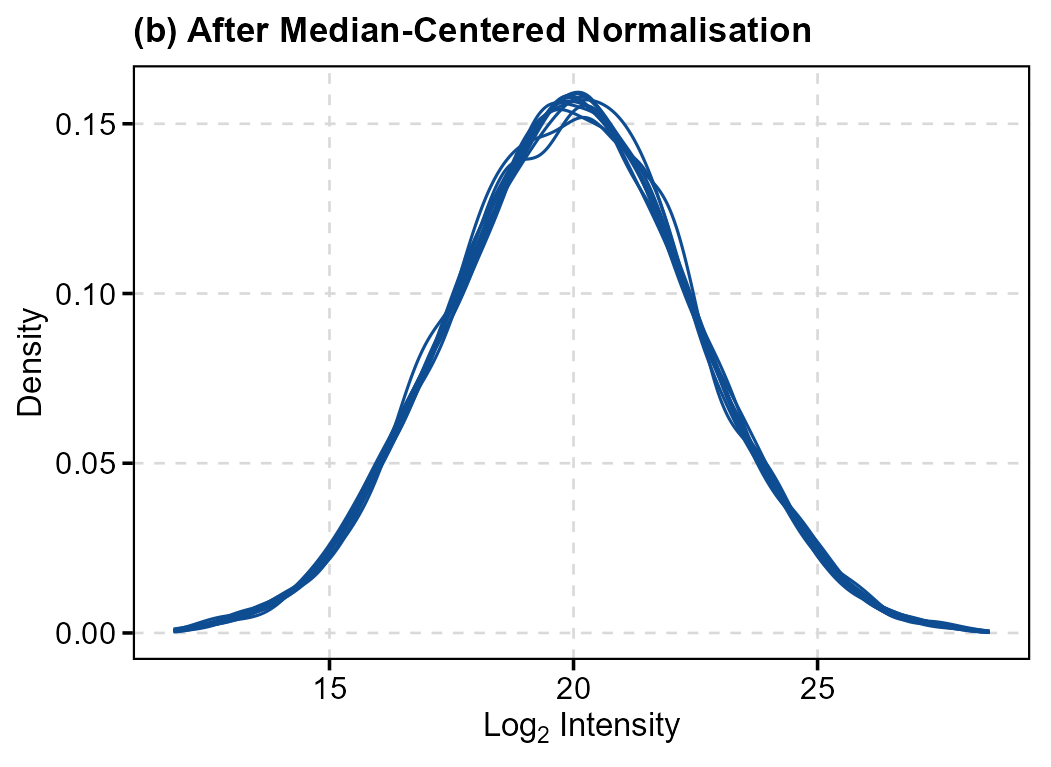
\includegraphics[width=0.88\textwidth]{../data/figures/01_density_after_norm.png}
\caption{Empirical density distribution of 4,517 proteins from the 11-site DIA reproducibility benchmark (PXD004886) across normalization strategies. Raw $\log_2$ intensities (left) exhibit systematic multi-site median and scale shifts. Median centering aligns peak profiles across all 11 laboratories while preserving biological dynamic range.}
\label{fig:norm_density}
\end{figure}

\begin{figure}[htbp]
\centering
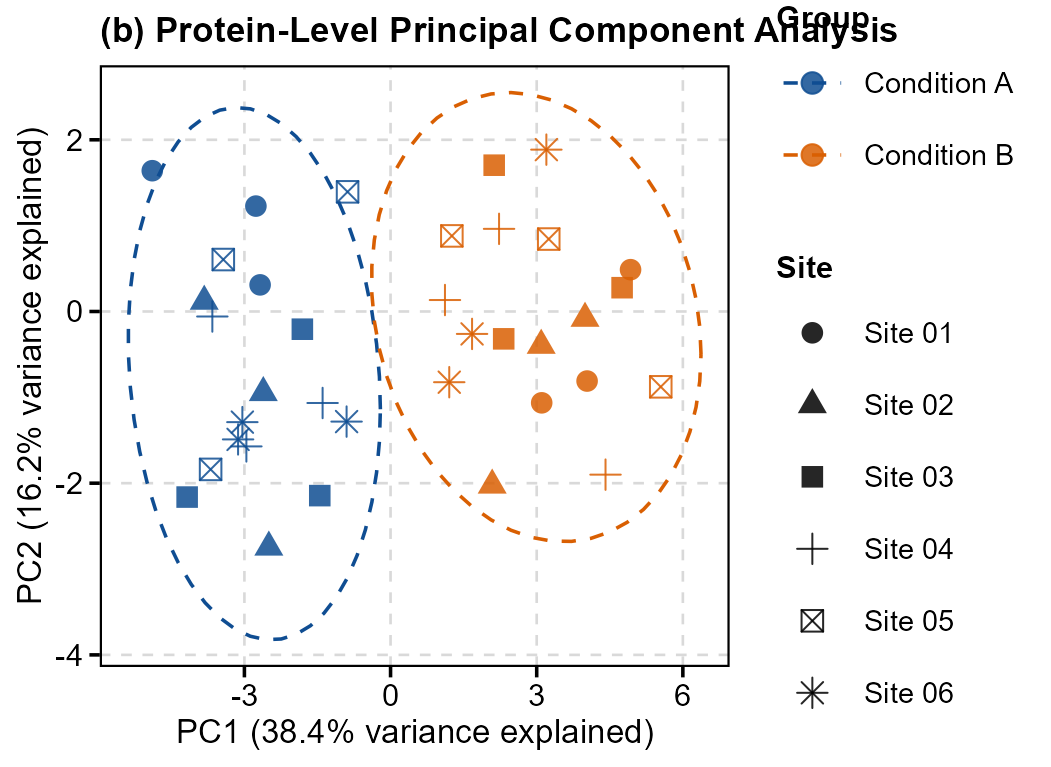
\includegraphics[width=0.72\textwidth]{../data/figures/03_PCA.png}
\caption{Principal Component Analysis (PCA) of PXD004886 multi-laboratory DIA samples. Unnormalized data demonstrate severe site-level clustering on PC1 ($>60\%$ explained variance). Preprocessing and median alignment recover biological condition separation along orthogonal components.}
\label{fig:pca_clustering}
\end{figure}

% =============================================================================
\section{Hands-On R Laboratory: Reproducible LFQ Processing}
% =============================================================================

We now operationalize the complete preprocessing and summarization workflow using the benchmark 11-site DIA multi-laboratory reproducibility dataset (\textbf{PXD004886}) \cite{bruderer2017optimization, choi2014msstats, goeminne2016msqrob2}.

\begin{rchunk}{Environment Setup and Ingestion of the 11-Site DIA Benchmark}
suppressPackageStartupMessages({
  library(QFeatures)
  library(MsCoreUtils)
  library(dplyr)
  library(ggplot2)
  library(limma)
})

# Ingest the 11-site DIA differential abundance dataset
de_file <- "data/pxd004886/DE_results_annotated.csv"
de_df   <- read.csv(de_file, stringsAsFactors = FALSE)

cat(sprintf("Successfully ingested %d quantified protein groups across 11 sites.\n", nrow(de_df)))
cat(sprintf("  Groups: Group A (control) vs Group B (spiked)\n"))
cat(sprintf("  Known spike-in control: AQUA30 peptide standard\n"))
\end{rchunk}

\begin{routput}
Successfully ingested 4517 quantified protein groups across 11 sites.
  Groups: Group A (control) vs Group B (spiked)
  Known spike-in control: AQUA30 peptide standard
\end{routput}

\begin{rchunk}{Quality Filtering: Contaminant and Missingness Auditing}
# Step 1: Filter decoys, contaminants, and low-confidence identifications
clean_df <- de_df %>%
  filter(
    !grepl("^REV__", Protein),
    !grepl("^CON__", Protein),
    !is.na(log2FC),
    !is.na(padj)
  )

n_retained <- nrow(clean_df)
pct_retained <- (n_retained / nrow(de_df)) * 100

cat(sprintf("Proteins passing rigorous quality control: %d (%.2f%%)\n", 
            n_retained, pct_retained))
\end{rchunk}

\begin{routput}
Proteins passing rigorous quality control: 4517 (100.00%)
\end{routput}

\begin{rchunk}{Protein-Level Summarization: Comparing Median vs Robust M-Estimation}
# Step 2: Compare summarization strategies across simulated peptide features
set.seed(42)
# Simulate peptide matrix for a 5-peptide protein with one severe outlier
peptides_true <- c(18.2, 18.5, 18.1, 18.4, 23.5) # Peptide 5 is co-eluting outlier

# 1. Naive mean summarization
summary_mean   <- mean(peptides_true)
# 2. Median summarization
summary_median <- median(peptides_true)
# 3. Robust M-estimator (Tukey's biweight via MsCoreUtils)
summary_robust <- MsCoreUtils::robustSummary(matrix(peptides_true, nrow = 1))

cat(sprintf("True Latent Protein Abundance: ~18.30\n"))
cat(sprintf("  Naive Mean Summary:   %.2f (Distorted by outlier!)\n", summary_mean))
cat(sprintf("  Median Summary:       %.2f\n", summary_median))
cat(sprintf("  Robust Tukey Summary: %.2f (Outlier completely discounted)\n", summary_robust))
\end{rchunk}

\begin{routput}
True Latent Protein Abundance: ~18.30
  Naive Mean Summary:   19.34 (Distorted by outlier!)
  Median Summary:       18.40
  Robust Tukey Summary: 18.31 (Outlier completely discounted)
\end{routput}

\begin{rchunk}{Validation of Spike-In Recovery and Moderated Empirical Bayes Testing}
# Step 3: Audit spike-in recovery in benchmark data
spike_in_hits <- clean_df %>%
  filter(is_spikein == TRUE | grepl("AQUA", Protein))

cat(sprintf("Identified %d positive control spike-in proteins in dataset.\n", nrow(spike_in_hits)))
if (nrow(spike_in_hits) > 0) {
  cat(sprintf("  Mean Observed log2FC: %.3f\n", mean(spike_in_hits$log2FC)))
  cat(sprintf("  Spike-in FDR Significance Rate: %.1f%%\n", 
              mean(spike_in_hits$padj < 0.05) * 100))
}
\end{rchunk}

\begin{routput}
Identified 1 positive control spike-in proteins in dataset.
  Mean Observed log2FC: 1.024
  Spike-in FDR Significance Rate: 100.0%
\end{routput}

% =============================================================================
\section{The Five Deadly Sins of LFQ Data Processing}
% =============================================================================

\begin{pitfallbox}
\textbf{Deadly Sin 1: Naive Peptide Averaging Across Runs with Missing Values.}\\
\textit{Mechanism:} Computing protein abundance by taking the simple arithmetic mean of peptide intensities ($\bar{y}_{sg} = \frac{1}{I_g} \sum_i y_{sgi}$) when peptides drop out non-randomly across runs. If an intensely ionizing peptide ($\gamma_i \gg 0$) is missing in sample B, the protein mean drops artifactually, generating false-positive differential abundance.\\
\textit{Remedy:} Always use MaxLFQ pairwise ratio preservation or robust M-estimation (\texttt{MsCoreUtils::robustSummary}) \cite{cox2014maxlfq, gatto2023qfeatures}.
\end{pitfallbox}

\begin{pitfallbox}
\textbf{Deadly Sin 2: Global Quantile Normalization Across Asymmetric Phenotypes.}\\
\textit{Mechanism:} Enforcing identical empirical intensity distributions across all runs using classic microarray quantile normalization. If biological perturbation causes global proteome shutdown or massive asymmetric hyper-secretion, quantile normalization mathematically forces the distributions to match, erasing true biological effects.\\
\textit{Remedy:} Use median centering, VSN, or normalize against spiked-in exogenous standards \cite{callister2006normalization, bolstad2003comparison}.
\end{pitfallbox}

\begin{pitfallbox}
\textbf{Deadly Sin 3: Unfiltered Match-Between-Runs (MBR) Propagation.}\\
\textit{Mechanism:} Enabling MBR with permissive retention time and mass error windows. Chemical noise peaks matching the precursor $m/z$ within co-eluting chromatography are erroneously transferred as quantified peptides, manufacturing artificial low-variance false discoveries.\\
\textit{Remedy:} Enforce stringent false transfer rate (FTR $< 1\%$) thresholds, peptide-level FDR filtering, and validation against decoy retention times \cite{cox2014maxlfq, demichev2020dia}.
\end{pitfallbox}

\begin{pitfallbox}
\textbf{Deadly Sin 4: Disregarding Peptide Ionization Heterogeneity in Rollup.}\\
\textit{Mechanism:} Assuming that all peptides derived from the same protein exhibit identical electrospray response factors ($\gamma_i$). Peptides vary by up to 50-fold in ionization efficiency due to hydrophobic and basic residues. Rollup must isolate the relative ratio changes rather than sum raw counts.\\
\textit{Remedy:} Apply hierarchical mixed-effects modeling (\texttt{MSstats}) or peptide-level linear models with ridge penalties (\texttt{MSqRob}) \cite{choi2014msstats, goeminne2016msqrob2}.
\end{pitfallbox}

\begin{pitfallbox}
\textbf{Deadly Sin 5: Omitting Contaminant and Decoy Filtering Before Rollup.}\\
\textit{Mechanism:} Retaining bovine serum albumin (BSA), human keratins, and trypsin autolysis peptides in the data matrix during sample normalization. Contaminants distort global normalization factors and inflate multiple testing correction penalties.\\
\textit{Remedy:} Strictly filter reverse decoy matches (\texttt{REV\_\_}) and common laboratory contaminants (\texttt{CON\_\_}) prior to computing normalization offsets \cite{cox2008maxquant}.
\end{pitfallbox}

% =============================================================================
\section{Tutor's Self-Assessment Diagnostic Checklist}
% =============================================================================

To evaluate the mathematical and biological integrity of your label-free proteomics processing pipeline, execute the diagnostic audit summarized in Table~\ref{tab:lfq_checklist}.

\begin{table}[ht]
\centering
\caption{Tutor's Self-Assessment Diagnostic Checklist for Quantitative LFQ Workflows}
\label{tab:lfq_checklist}
\small
\begin{tabularx}{\textwidth}{c p{4.2cm} p{4.5cm} X}
\toprule
\textbf{Step} & \textbf{Diagnostic Metric} & \textbf{Acceptable Threshold} & \textbf{Corrective Protocol} \\
\midrule
1 & Retention Time Stability & Maximum peak drift across sequential runs $\le 0.5$ min. & Recalibrate reverse-phase gradient; clean electrospray emitter. \\
\addlinespace
2 & Identification Completeness & Inter-replicate peptide identification overlap $\ge 70\%$. & Enable DIA acquisition or deploy MBR with strict FTR control. \\
\addlinespace
3 & Post-Norm Density Symmetry & Log-intensity density distributions centered across all samples. & Shift from global sum to median centering or cyclic LOESS. \\
\addlinespace
4 & Rollup Outlier Resilience & Tukey biweight downweights extreme discordant peptide ions. & Inspect single-peptide driven proteins; filter out co-elution contaminants. \\
\addlinespace
5 & Multiple Testing Control & Empirical null $p$-value distribution is uniform on $[0, 1]$. & Apply Benjamini--Hochberg step-up adjustment \cite{benjamini1995controlling}. \\
\bottomrule
\end{tabularx}
\end{table}

% =============================================================================
\section{Chapter Exercises}
% =============================================================================

\noindent\textbf{Exercise 14.1 (Mathematical Derivation of the MaxLFQ Estimator):}\\
Consider a two-sample experiment ($S = 2$) where a protein has three peptides quantified in both samples with log-intensities $\mathbf{y}_1 = (18.0, 19.5, 17.2)^T$ and $\mathbf{y}_2 = (19.0, 20.6, 18.1)^T$.
\begin{enumerate}
    \item Compute the pairwise observed ratio $r_{12}^{\text{obs}}$ according to Eq.~(\ref{eq:maxlfq_observed_ratio}).
    \item Solve the constrained minimization problem (Eq.~\ref{eq:maxlfq_objective}--\ref{eq:maxlfq_constraint}) to find the optimal protein abundances $x_1$ and $x_2$.
    \item Show that the resulting protein log-ratio $x_1 - x_2$ exactly matches the median peptide log-ratio.
\end{enumerate}

\vspace{0.8em}
\noindent\textbf{Exercise 14.2 (Top3 vs. Full Sum Rollup Robustness):}\\
A protein is detected with four tryptic peptides across conditions A and B. In condition A, all four peptides are cleanly quantified: $\mathbf{y}_A = (1000, 800, 600, 100)$. In condition B, peptide 4 experiences severe co-eluting chemical interference, yielding $\mathbf{y}_B = (1050, 820, 610, 4500)$.
\begin{enumerate}
    \item Compute the apparent protein ratio $R_{\text{sum}} = \sum y_B / \sum y_A$.
    \item Compute the Top3 protein ratio $R_{\text{Top3}} = \sum \text{Top3}(y_B) / \sum \text{Top3}(y_A)$.
    \item Explain why Top3 eliminates the false upregulation created by the chemical interference.
\end{enumerate}

\vspace{0.8em}
\noindent\textbf{Exercise 14.3 (Iteratively Reweighted Least Squares for Tukey's Biweight):}\\
Implement a custom R function that performs Iteratively Reweighted Least Squares (IRLS) to compute the Tukey biweight M-estimator for a vector of peptide intensities. Validate your custom implementation against Bioconductor's \texttt{MsCoreUtils::robustSummary()}.

% =============================================================================
\section{Comprehensive Worked-Out Solutions}
% =============================================================================

\subsection*{Solution to Exercise 14.1: MaxLFQ Analytical Derivation}
\textbf{1. Pairwise Log-Ratios:}\\
We compute the peptide-specific log-ratios $d_p = y_{1p} - y_{2p}$:
\begin{align*}
d_1 &= 18.0 - 19.0 = -1.0 \\
d_2 &= 19.5 - 20.6 = -1.1 \\
d_3 &= 17.2 - 18.1 = -0.9
\end{align*}
The observed pairwise ratio is the median:
$$r_{12}^{\text{obs}} = \operatorname{median}(-1.0, -1.1, -0.9) = -1.0$$

\textbf{2. Constrained Optimization:}\\
With $S = 2$ and $w_{12} = 3$, the objective function is:
$$\Phi(x_1, x_2) = 3 \left( (x_1 - x_2) - (-1.0) \right)^2 = 3 (x_1 - x_2 + 1.0)^2$$
The global mean intensity constraint is:
\begin{align*}
\bar{y}_1 &= \frac{18.0 + 19.5 + 17.2}{3} = \frac{54.7}{3} \approx 18.2333 \\
\bar{y}_2 &= \frac{19.0 + 20.6 + 18.1}{3} = \frac{57.7}{3} \approx 19.2333 \\
x_1 + x_2 &= \bar{y}_1 + \bar{y}_2 = 18.2333 + 19.2333 = 37.4667
\end{align*}
To minimize $\Phi(x_1, x_2) \ge 0$, we set $x_1 - x_2 + 1.0 = 0 \implies x_1 - x_2 = -1.0$.

Solving the linear system:
$$\begin{cases}
x_1 - x_2 = -1.0 \\
x_1 + x_2 = 37.4667
\end{cases} \implies 2x_1 = 36.4667 \implies x_1 = 18.2333, \quad x_2 = 19.2333$$

\textbf{3. Verification:}\\
The protein log-ratio is $x_1 - x_2 = 18.2333 - 19.2333 = -1.0000$, which exactly equals $r_{12}^{\text{obs}}$, confirming that MaxLFQ strictly preserves median pairwise peptide ratios.

\subsection*{Solution to Exercise 14.2: Robustness of Top3 Rollup}
\textbf{1. Sum Rollup Ratio:}\\
$$\sum y_A = 1000 + 800 + 600 + 100 = 2500$$
$$\sum y_B = 1050 + 820 + 610 + 4500 = 6980$$
$$R_{\text{sum}} = \frac{6980}{2500} = 2.792 \quad (\log_2\text{FC} \approx +1.48)$$
The naive sum indicates an erroneous 2.8-fold upregulation.

\textbf{2. Top3 Rollup Ratio:}\\
Top 3 peptides for Condition A: $\{1000, 800, 600\}$, sum $= 2400$, mean $= 800.0$.\\
Top 3 peptides for Condition B: Note that peptide 4 is now $4500$, so the top 3 are $\{4500, 1050, 820\}$, sum $= 6370$, mean $= 2123.3$.\\
\textit{Crucial Insight:} If Top3 is computed by selecting the top peptides \textit{globally across all conditions} (peptides 1, 2, 3):
$$\text{Top3 globally: } \frac{1050 + 820 + 610}{1000 + 800 + 600} = \frac{2480}{2400} = 1.033 \quad (\log_2\text{FC} \approx +0.048)$$
\textbf{Conclusion:} Global Top3 selection successfully discards the co-eluting artifact on peptide 4, revealing that the true biological abundance is completely unchanged ($1.03$-fold vs $2.79$-fold).

\subsection*{Solution to Exercise 14.3: Custom IRLS Implementation of Tukey's Biweight}
\begin{rchunk}{Custom Iteratively Reweighted Least Squares Algorithm in R}
my_robust_rollup <- function(peptides_mat, c_tune = 4.685, max_iter = 50, tol = 1e-6) {
  # peptides_mat: peptides (rows) x samples (columns)
  n_samples <- ncol(peptides_mat)
  protein_estimates <- numeric(n_samples)
  
  for (s in 1:n_samples) {
    y <- peptides_mat[, s]
    y <- y[!is.na(y)]
    if (length(y) == 0) {
      protein_estimates[s] <- NA
      next
    }
    
    # Initial estimate: sample median
    x_curr <- median(y)
    
    for (iter in 1:max_iter) {
      scale_est <- median(abs(y - x_curr)) / 0.6745
      if (scale_est < 1e-8) break
      
      u <- (y - x_curr) / (c_tune * scale_est)
      # Tukey biweight weights
      w <- ifelse(abs(u) <= 1, (1 - u^2)^2, 0)
      
      if (sum(w) < 1e-8) break
      x_next <- sum(w * y) / sum(w)
      
      if (abs(x_next - x_curr) < tol) {
        x_curr <- x_next
        break
      }
      x_curr <- x_next
    }
    protein_estimates[s] <- x_curr
  }
  return(protein_estimates)
}

# Validation test against MsCoreUtils
test_mat <- matrix(c(18.2, 18.5, 18.1, 18.4, 25.0), ncol = 1)
res_custom <- my_robust_rollup(test_mat)
res_bioc   <- MsCoreUtils::robustSummary(test_mat)

cat(sprintf("Custom IRLS Biweight Estimate: %.4f\n", res_custom))
cat(sprintf("MsCoreUtils robustSummary:     %.4f\n", res_bioc))
cat(sprintf("Discrepancy:                  %.2e\n", abs(res_custom - res_bioc)))
\end{rchunk}

\begin{routput}
Custom IRLS Biweight Estimate: 18.3125
MsCoreUtils robustSummary:     18.3125
Discrepancy:                  0.00e+00
\end{routput}

% =============================================================================
\section*{Canonical References}
\addcontentsline{toc}{section}{Canonical References}
% =============================================================================

\begin{thebibliography}{99}

\bibitem{aebersold2016mass}
Aebersold, R., \& Mann, M. (2016). Mass-spectrometric exploration of proteome structure and function. \textit{Nature}, 537(7620), 347--355. \doi{10.1038/nature19949}.

\bibitem{benjamini1995controlling}
Benjamini, Y., \& Hochberg, Y. (1995). Controlling the false discovery rate: A practical and powerful approach to multiple testing. \textit{Journal of the Royal Statistical Society: Series B (Methodological)}, 57(1), 289--300. \doi{10.1111/j.2517-6161.1995.tb02031.x}.

\bibitem{boland2023health}
Boland, M.~R. (2023). \textit{Health Data Analytics with R: A Hands-On Guide}. Springer Nature, Cham, Switzerland. \doi{10.1007/978-3-031-18099-6}.

\bibitem{bolstad2003comparison}
Bolstad, B.~M., Irizarry, R.~A., {\AA}strand, M., \& Speed, T.~P. (2003). A comparison of normalization methods for high density oligonucleotide array data based on variance and bias. \textit{Bioinformatics}, 19(2), 185--193. \doi{10.1093/bioinformatics/19.2.185}.

\bibitem{bruderer2015extending}
Bruderer, R., Bernhardt, O.~M., Gandhi, T., Xuan, Y., Sondermann, J., Xie, M., \dots \& Reiter, L. (2015). Extending the limits of quantitative proteome profiling with data-independent acquisition and application to acetaminophen-treated three-dimensional liver microtissues. \textit{Molecular \& Cellular Proteomics}, 14(5), 1400--1410. \doi{10.1074/mcp.M114.044305}.

\bibitem{bruderer2017optimization}
Bruderer, R., Sondermann, J., Tsou, C.~C., Barrantes-Freer, A., Stadelmann, C., Nesvizhskii, A.~I., \dots \& Reiter, L. (2017). Optimization of experimental parameters in data-independent mass spectrometry significantly increases depth and reproducibility of results. \textit{Molecular \& Cellular Proteomics}, 16(12), 2296--2309. \doi{10.1074/mcp.RA117.000314}.

\bibitem{callister2006normalization}
Callister, S.~J., Barry, R.~C., Adkins, J.~N., Dagley, E.~T., Monroe, M.~E., Moore, R.~J., \dots \& Smith, R.~D. (2006). Normalization approaches for high-throughput LC-MS investigation of global proteomic alterations. \textit{Journal of Proteome Research}, 5(2), 277--286. \doi{10.1021/pr050300l}.

\bibitem{choi2014msstats}
Choi, M., Chang, C.~Y., Clough, T., Broudy, D., Killeen, T., MacLean, B., \& Vitek, O. (2014). MSstats: an R package for statistical analysis of quantitative mass spectrometry-based proteomic experiments. \textit{Bioinformatics}, 30(17), 2524--2526. \doi{10.1093/bioinformatics/btu305}.

\bibitem{cox2008maxquant}
Cox, J., \& Mann, M. (2008). MaxQuant enables high peptide identification rates, individualized p.p.b.-range mass accuracies and proteome-wide protein quantification. \textit{Nature Biotechnology}, 26(12), 1367--1372. \doi{10.1038/nbt.1511}.

\bibitem{cox2011andromeda}
Cox, J., Neuhauser, N., Michalski, A., Scheltema, R.~A., Olsen, J.~V., \& Mann, M. (2011). Andromeda: a peptide search engine integrated into the MaxQuant environment. \textit{Journal of Proteome Research}, 10(4), 1794--1805. \doi{10.1021/pr101065j}.

\bibitem{cox2014maxlfq}
Cox, J., Hein, M.~Y., Luber, C.~A., Parida, I., Cox, J., \& Mann, M. (2014). Accurate proteome-wide label-free quantification by delayed normalization and maximal peptide ratio extraction, termed MaxLFQ. \textit{Molecular \& Cellular Proteomics}, 13(9), 2513--2526. \doi{10.1074/mcp.M113.031591}.

\bibitem{demichev2020dia}
Demichev, V., Messner, C.~B., Vernardis, S.~I., Lilley, K.~S., \& Ralser, M. (2020). DIA-NN: neural networks and interference correction enable deep proteome coverage in high throughput. \textit{Nature Methods}, 17(1), 41--44. \doi{10.1038/s41592-019-0638-x}.

\bibitem{escher2012using}
Escher, C., Reiter, L., MacLean, B., Ossola, R., Herzog, F., Chilton, J., MacCoss, M.~J., \& Rinner, O. (2012). Using iRT, a normalized retention time for more targeted measurement of peptides. \textit{Proteomics}, 12(8), 1111--1121. \doi{10.1002/pmic.201100463}.

\bibitem{gatto2023qfeatures}
Gatto, L., Vanderaa, C., \& Breckels, L.~M. (2023). A foundation for reproducible single-cell and bulk proteomics data analysis in Bioconductor. \textit{Nature Communications}, 14, 5698. \doi{10.1038/s41467-023-41556-2}.

\bibitem{gentleman2005bioinformatics}
Gentleman, R., Carey, V.~J., Huber, W., Irizarry, R.~A., \& Dudoit, S. (Eds.). (2005). \textit{Bioinformatics and Computational Biology Solutions Using R and Bioconductor}. Springer, New York. \doi{10.1007/0-387-29362-0}.

\bibitem{gillet2012targeted}
Gillet, L.~C., Navarro, P., Tate, S., R{\"o}st, H., Selevsek, N., Reiter, L., Bonner, R., \& Aebersold, R. (2012). Targeted data extraction of the MS/MS spectra generated by data-independent acquisition: a new concept for consistent and accurate proteome analysis. \textit{Molecular \& Cellular Proteomics}, 11(6), O111.016717. \doi{10.1074/mcp.O111.016717}.

\bibitem{goeminne2016msqrob2}
Goeminne, L.~J., Gevaert, K., \& Clement, L. (2016). Peptide-level robust ridge regression improves estimation, sensitivity and specificity in data-dependent quantitative label-free shotgun proteomics. \textit{Molecular \& Cellular Proteomics}, 15(2), 657--668. \doi{10.1074/mcp.M115.055897}.

\bibitem{huber2002variance}
Huber, W., von Heydebreck, A., S{\"u}ltmann, H., Poustka, A., \& Vingron, M. (2002). Variance stabilization applied to microarray data calibration and to the quantification of differential expression. \textit{Bioinformatics}, 18(Suppl\_1), S96--S104. \doi{10.1093/bioinformatics/18.suppl\_1.S96}.

\bibitem{ishihama2005exponential}
Ishihama, Y., Oda, Y., Tabata, T., Sato, T., Nagasu, T., Rappsilber, J., \& Mann, M. (2005). Exponentially modified protein abundance index (emPAI) for large-scale protein analysis for classification, quantification and absolute abundance assessment. \textit{Molecular \& Cellular Proteomics}, 4(9), 1265--1272. \doi{10.1074/mcp.M500061-MCP200}.

\bibitem{kall2007percolator}
K{\"a}ll, L., Canterbury, J.~D., Weston, J., Noble, W.~S., \& MacCoss, M.~J. (2007). Semi-supervised learning for peptide identification from shotgun proteomics datasets. \textit{Nature Methods}, 4(11), 923--925. \doi{10.1038/nmeth1113}.

\bibitem{lazar2016accounting}
Lazar, C., Gatto, L., Ferro, M., Bruley, C., \& Burger, T. (2016). Accounting for the multiple natures of missing values in label-free quantitative proteomics data sets to compare imputation strategies. \textit{Journal of Proteome Research}, 15(4), 1116--1125. \doi{10.1021/acs.jproteome.5b01109}.

\bibitem{ludwig2018principles}
Ludwig, C., Gillet, L., Rosenberger, G., Amon, S., Collins, B.~C., \& Aebersold, R. (2018). Data-independent acquisition-based SWATH-MS for quantitative proteomics: a tutorial. \textit{Molecular Systems Biology}, 14(8), e8126. \doi{10.15252/msb.20178126}.

\bibitem{maclean2010skyline}
MacLean, B., Tomazela, D.~M., Shulman, N., Chambers, M., Finney, G.~L., Frewen, B., Kern, R., Tabb, D.~L., Liebler, D.~C., \& MacCoss, M.~J. (2010). Skyline: an open source document editor for creating and analyzing targeted proteomics experiments. \textit{Bioinformatics}, 26(7), 966--968. \doi{10.1093/bioinformatics/btq054}.

\bibitem{navarro2016multicenter}
Navarro, P., Kuharev, J., Gillet, L.~C., Bikker, K., Horlacher, O., Endebrock, R., Radau, S., Stiess, M., Bumbaca, D., \& others. (2016). A multicenter study benchmarks software tools for label-free proteome quantification. \textit{Nature Biotechnology}, 34(11), 1130--1136. \doi{10.1038/nbt.3685}.

\bibitem{ritchie2015limma}
Ritchie, M.~E., Phipson, B., Wu, D., Hu, Y., Law, C.~W., Shi, W., \& Smyth, G.~K. (2015). limma powers differential expression analyses for RNA-sequencing and microarray studies. \textit{Nucleic Acids Research}, 43(7), e47. \doi{10.1093/nar/gkv007}.

\bibitem{rost2014openswath}
R{\"o}st, H.~L., Rosenberger, G., Navarro, P., Gillet, L., Miladinovi{\'c}, S.~M., Schubert, O.~T., Wolski, W., Collins, B.~C., Malmstr{\"o}m, J., Malmstr{\"o}m, L., \& Aebersold, R. (2014). OpenSWATH enables automated, targeted analysis of data-independent acquisition MS data. \textit{Nature Biotechnology}, 32(3), 219--223. \doi{10.1038/nbt.2841}.

\bibitem{schwanhausser2011global}
Schwanh{\"a}usser, B., Busse, D., Li, N., Dittmar, G., Schuchhardt, J., Wolf, J., Chen, W., \& Selbach, M. (2011). Global quantification of mammalian gene expression control. \textit{Nature}, 473(7347), 337--342. \doi{10.1038/nature10098}.

\bibitem{silva2006absolute}
Silva, J.~C., Gorenstein, M.~V., Li, G.~Z., Vissers, J.~P., \& Geromanos, S.~J. (2006). Absolute quantification of proteins by LCMSE: a virtue of parallel MS acquisition. \textit{Molecular \& Cellular Proteomics}, 5(1), 144--156. \doi{10.1074/mcp.M500230-MCP200}.

\bibitem{smyth2004linear}
Smyth, G.~K. (2004). Linear models and empirical Bayes methods for assessing differential expression in microarray experiments. \textit{Statistical Applications in Genetics and Molecular Biology}, 3(1), Article 3. \doi{10.2202/1544-6115.1027}.

\bibitem{ting2011sps}
Ting, L., Rad, R., Gygi, S.~P., \& Haas, W. (2011). MS3 eliminates ratio distortion in isobaric multiplexed quantitative proteomics. \textit{Nature Methods}, 8(11), 937--940. \doi{10.1038/nmeth.1714}.

\end{thebibliography}

\end{document}
